\section{Introducción}
Para realizar esta práctica final hemos elegido hacer una página web publicitaria de Nueva Zelanda, cuyo objetivo sería el de publicitar algunas actividades del país.

Hemos aplicado los conocimientos aprendidos tanto en la asignatura de Interacción Persona-Ordenador, Desarrollo de Aplicaciones Web, y de la propia Multimedia.\\

La página está alojada en \href{http://visitnznow.esy.es/}{http://visitnznow.esy.es/}
\section{Decisiones de diseño}
\subsection{Estructura del código}
Siguiendo los requisitos que se especificaban en el enunciado, la página está compuesta de 4 ficheros .html, junto con su correspondiente hoja de estilo.Los archivos son:
\begin{itemize}
	\item \textbf{index.html: }página de bienvenida. Contiene un menú superior para la navegación y un footer que están presente en el resto de las vistas. Tiene también las opiniones de algunos supuestos clientes, así como algunas gráficas de satisfacción. Tiene disponible un pequeño reproductor de audio para escuchar el audio ne Nueva Zelanda. 
	\item \textbf{places-to-visit.html: } se muestran algunas fotos de Nueva Zelanda, así como un pequeño vídeo de presentación de sus lugares más famosos. También tiene un pequeño navegador de Google Maps.
	\item \textbf{where-eat.html: }un listado con loas opciones disponibles a la hora de elegir restaurante. Tiene una animación con una presentación gastronómica.
	\item \textbf{contact.html: }Permite enviar una postal a un amigo. Puedes elegir una foto de la galería y escribir el cuerpo del mensaje. Finalmente tienes que especificar el nombre y la dirección de correo del destinatario.
\end{itemize}

\subsection{Decisiones para accesibilidad}

Aunque en un principio pensamos un diseño con numerosos efectos, carruseles y animaciones, éstos no eran compatibles con conseguir una web accesible. Así que finalmente optamos por quitar todos estos efectos, pero tratando de mantener una presentación agradable y moderna.
A la hora de pasar las validaciones de la W3C nos percatamos de los numerosos errores que habíamos cometido, por lo que tuvimos que quitar prácticamente los efectos que nos quedaban.
\clearpage

\subsection{Decisiones para responsive}
La página utiliza el framework de html \textit{Bootstrap} para que la página sea responsive. La estructura de las columnas, así como el menú de navegación superior, se colapsan en caso de que se acceda a la página a través de un dispositivo con menor tamaño de pantalla.
\section{Resultados de la validación}
\subsection{Resultados obtenidos}

\subsubsection{Accesibilidad}
Tras la validaciones pertinentes, hemos conseguido que nuestra página tenga un nivel \textbf{AAA}. Para validar nuestra página hemos usado 2 de la herramientas propuestas en el enunciado: \textit{Examinator} y \textit{TAW}:

\begin{enumerate}
	\item \textbf{index.html: }nota examinator: \textbf{10}. Errores en TAW: \textbf{1} (no reconoce el audio).	
	\item \textbf{places-to-visit.html: }nota examinator: \textbf{10}. Errores en TAW: \textbf{0} 
	\item \textbf{where-eat.html: }nota examinator: \textbf{10}. Errores en TAW: \textbf{0}
	\item \textbf{contact.html: }nota examinator: \textbf{10}. Errores en TAW: \textbf{1}(no reconoce que la página esté en español)

\end{enumerate}
	\begin{figure}
		\centering
		\begin{subfigure}{.5\textwidth}
			\centering
			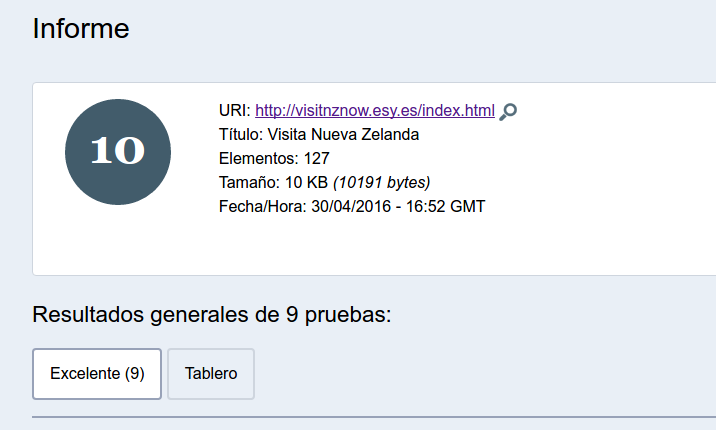
\includegraphics[width=.8\linewidth]{./Fotos/exa-index.png}
			\caption{Examinator}
			\label{fig: Examinator index}
		\end{subfigure}%
		\begin{subfigure}{.5\textwidth}
			\centering
			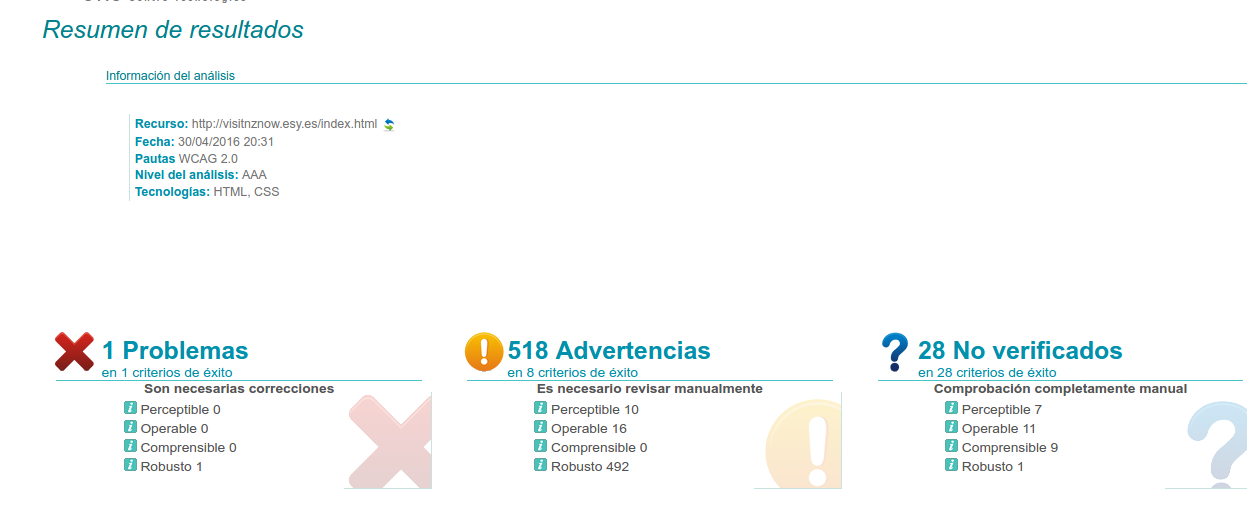
\includegraphics[width=.8\linewidth]{./Fotos/taw-index.png}
			\caption{TAW}
			\label{fig: TAW index}
		\end{subfigure}
		\caption{Resultados accesibilidad index}
		\label{fig: Resultados accesibilidad index}
	\end{figure}
		\begin{figure}
			\centering
			\begin{subfigure}{.5\textwidth}
				\centering
				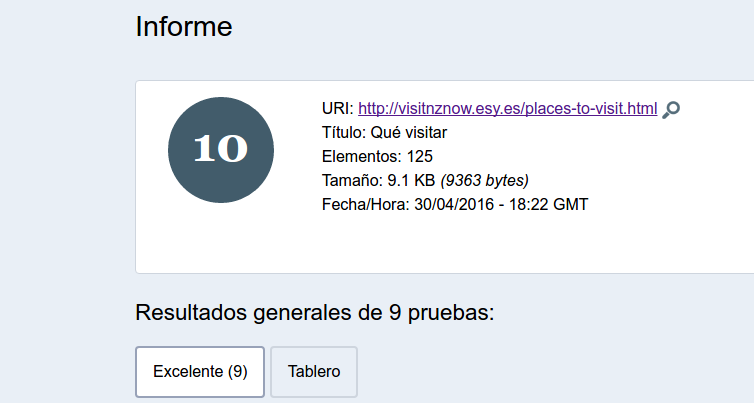
\includegraphics[width=.8\linewidth]{./Fotos/exa-visit.png}
				\caption{Examinator}
				\label{fig: Examinator places-to-visit}
			\end{subfigure}%
			\begin{subfigure}{.5\textwidth}
				\centering
				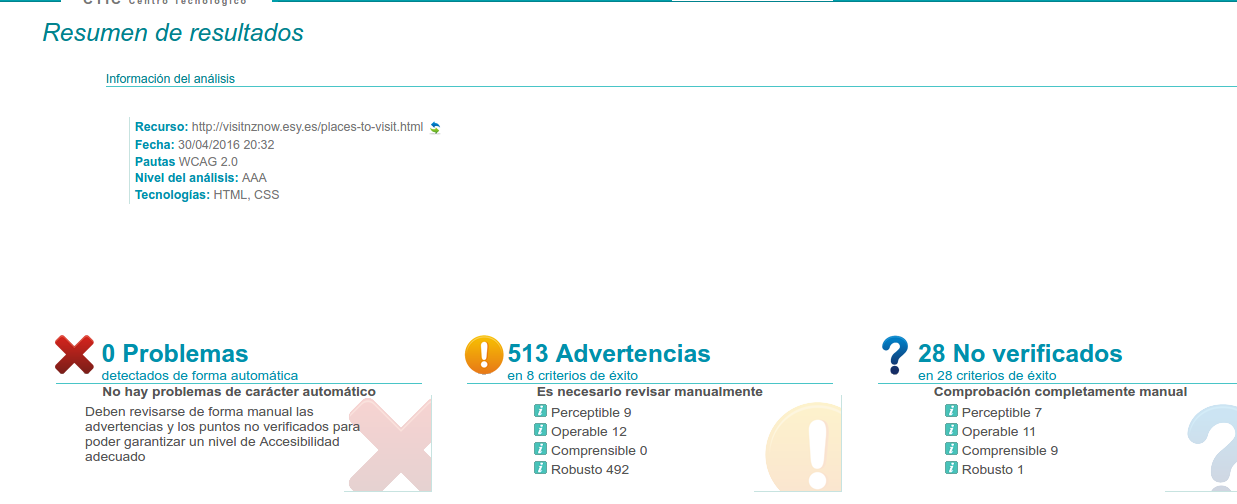
\includegraphics[width=.8\linewidth]{./Fotos/taw-visit.png}
				\caption{TAW}
				\label{fig: TAW places-to-visit}
			\end{subfigure}
			\caption{Resultados accesibilidad places-to-visit}
			\label{fig: Resultados accesibilidad places-to-visit}
		\end{figure}


	\begin{figure}
		\centering
		\begin{subfigure}{.5\textwidth}
			\centering
			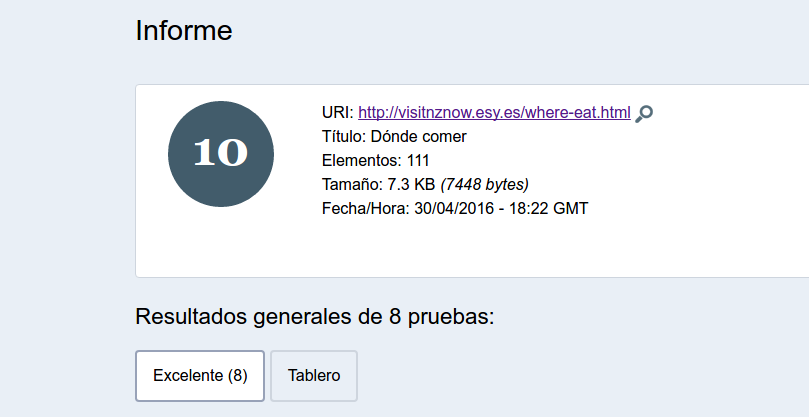
\includegraphics[width=.8\linewidth]{./Fotos/exa-eat.png}
			\caption{Examinator}
			\label{fig: Examinator where-eat}
		\end{subfigure}%
		\begin{subfigure}{.5\textwidth}
			\centering
			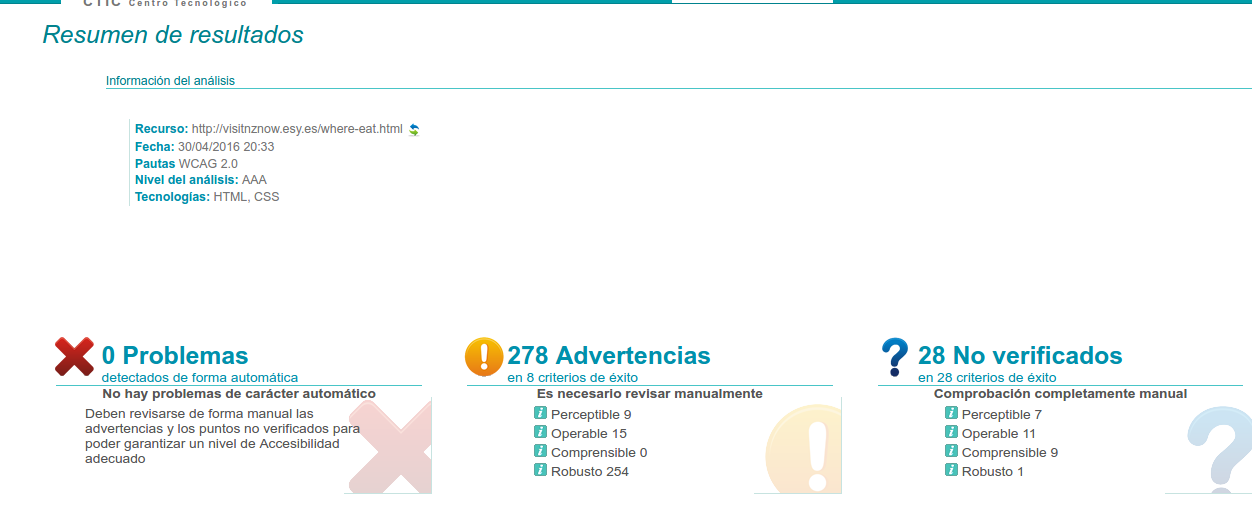
\includegraphics[width=.8\linewidth]{./Fotos/taw-eat.png}
			\caption{TAW}
			\label{fig: TAW where-eat}
		\end{subfigure}
		\caption{Resultados accesibilidad where-eat}
		\label{fig:Resultados accesibilidad where-eat}
	\end{figure}
		\begin{figure}
			\centering
			\begin{subfigure}{.5\textwidth}
				\centering
				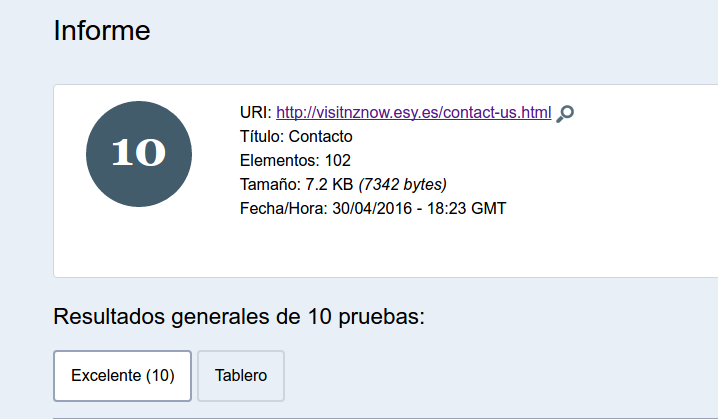
\includegraphics[width=.8\linewidth]{./Fotos/exa-contact.png}
				\caption{Examinator}
				\label{fig: Examinator contact}
			\end{subfigure}%
			\begin{subfigure}{.5\textwidth}
				\centering
				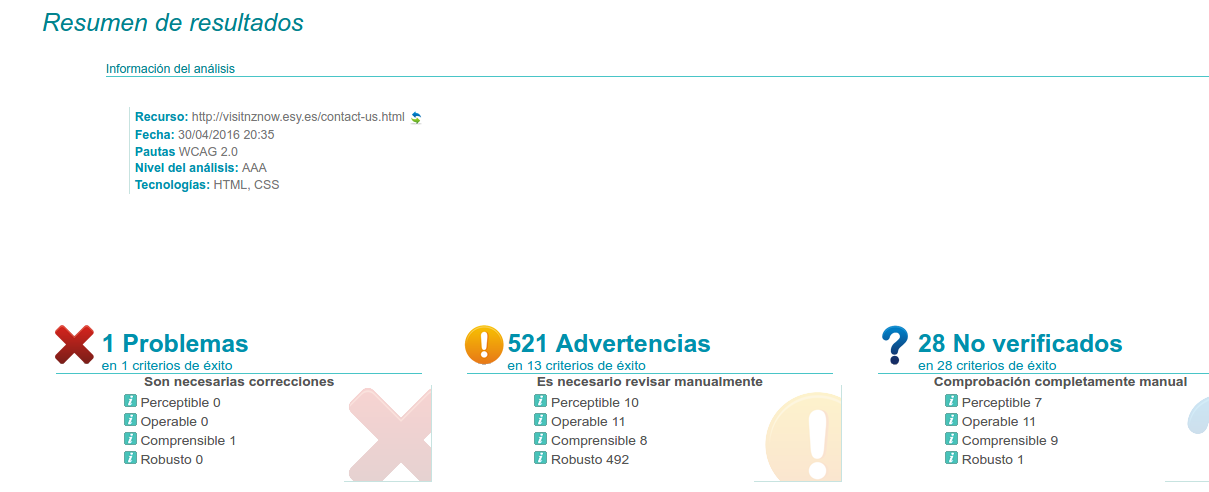
\includegraphics[width=.8\linewidth]{./Fotos/taw-contact.png}
				\caption{TAW}
				\label{fig: TAW contactsub2}
			\end{subfigure}
			\caption{Resultados accesibilidad contact}
			\label{fig: Resultados accesibilidad contact}
		\end{figure}
\clearpage
\subsubsection{Multinavegador y multiplataforma}
Los resultados multinavegador se presentarán en la sección de Tabla comparativa.\\
Para comprobar el diseño responsive hemos utilizado la opción disponible en las herramientas para desarrolladores de Google Chrome, así como \textit{responsinator} y nuestros propios smartphones. El resultado ha sido satisfactorio para todas las vistas.

\begin{figure}[h]
	\centering
	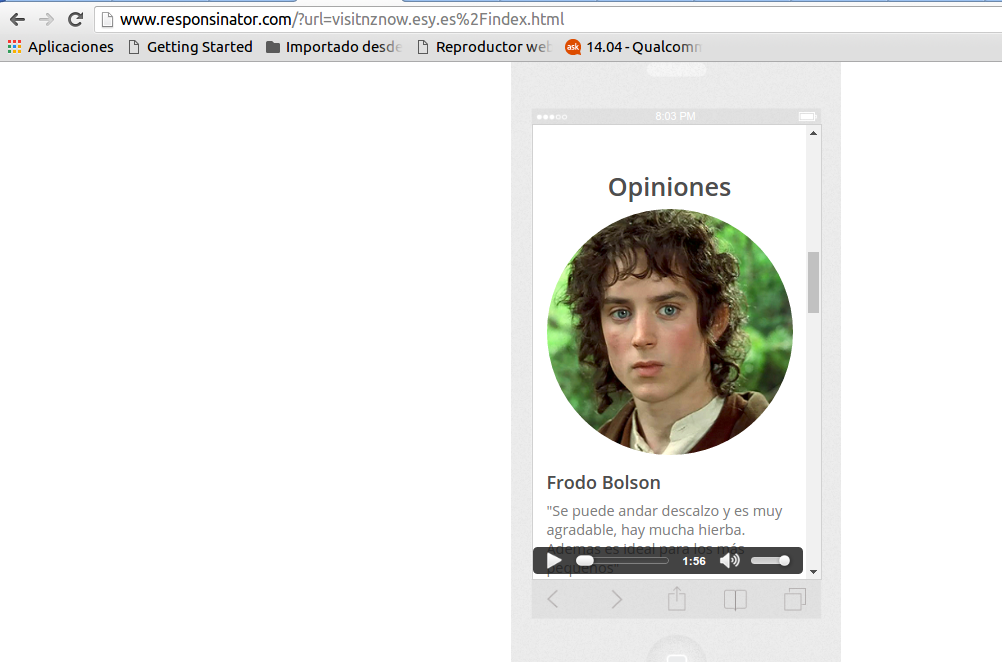
\includegraphics[width=0.50\textwidth]{./Fotos/responsinator.png}
	\caption{Responsinator}
	\label{fig: Responsinator}
\end{figure}

\subsubsection{iPhone e iPad}
Tras comprobar con las herramientas \textit{TestiPhone} y \textbf{Movile Test me}, podemos cerciorarnos que la página se ve correctamente en los dispositivos MAC:
\begin{figure}[h]
	\centering
	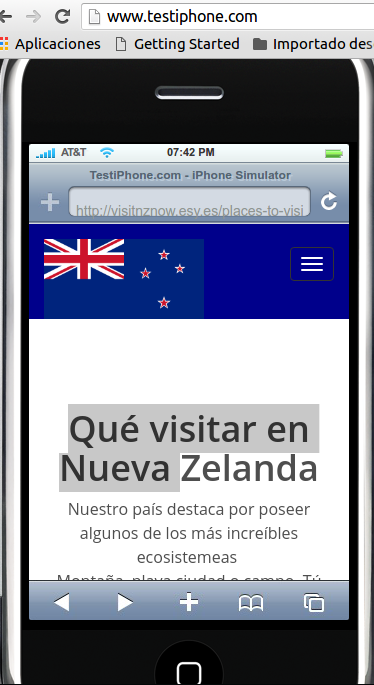
\includegraphics[height=0.50\textwidth]{./Fotos/testiphone.png}
	\caption{testIphone}
	\label{fig: testIphone}
\end{figure}


\subsubsection{Navegación textual}
Hemos usado el \textit{Emulador Lynx Viewer}:

\begin{figure}[h]
	\centering
	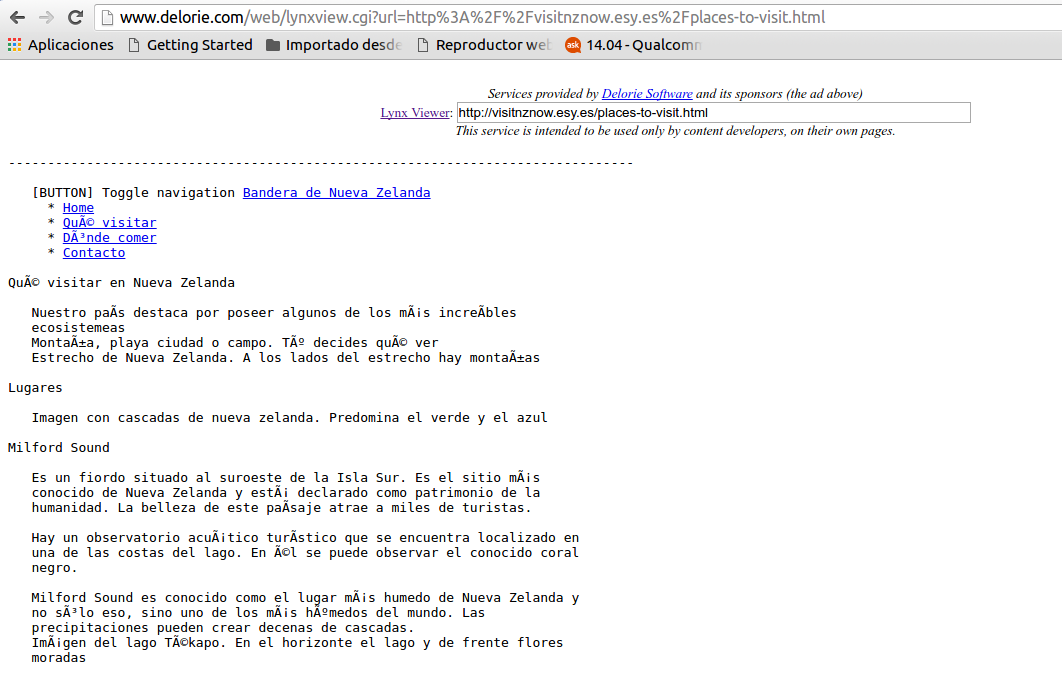
\includegraphics[width=0.50\textwidth]{./Fotos/lynx.png}
	\caption{Lynx}
	\label{fig: Resultados del Lynx}
\end{figure}


\subsubsection{Peso y velocidad de carga}
Para analizar los tiempos de carga hemos analizado la vista que tiene el mayor número de imágenes:
\begin{figure}[h]
	\centering
	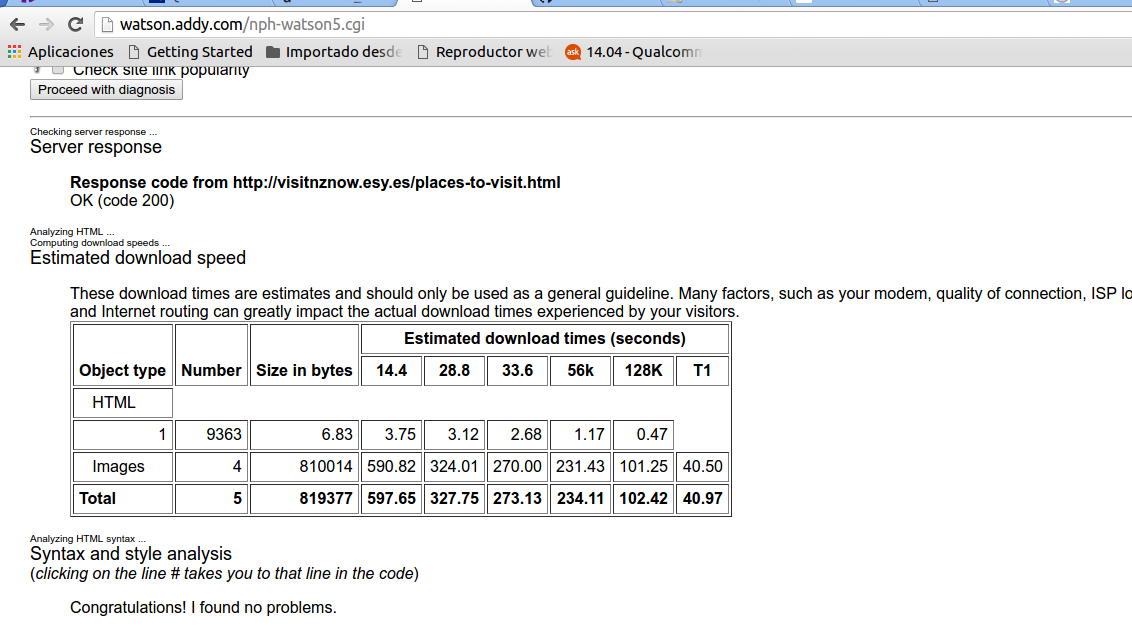
\includegraphics[width=0.50\textwidth]{./Fotos/watson.png}
	\caption{Resultados del Watson}
	\label{fig: Resultados del Watson}
\end{figure}
Aunque el tiempo de carga puede llegar a ser elevado (medio segundo para conexiones muy lentas), hay que tener en cuenta que la página al tener como propósito mostrar imágenes de Nueva Zelanda, éstas deben tener una muy buena calidad de imagen.
\clearpage
\subsubsection{Buscadores}
\begin{figure}[h]
	\centering
	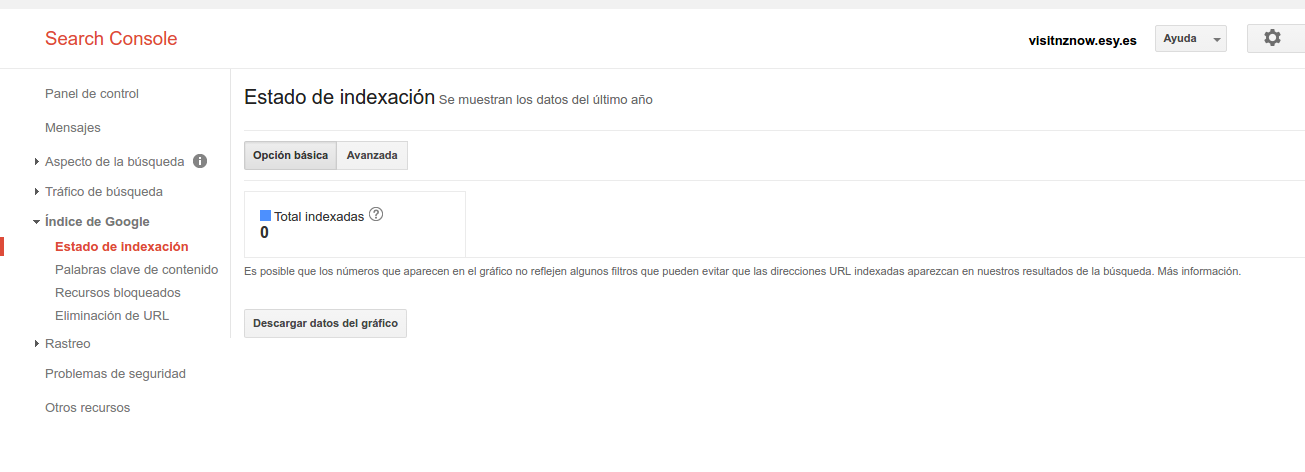
\includegraphics[width=0.50\textwidth]{./Fotos/indexacion.png}
	\caption{Indexación en Google}
	\label{fig: Indexación en Google}
\end{figure}
Debido a que el servidor gratuito que hemos elegido (Hostinger) tarda unos días en posicionar la página y que no hemos hecho un análisis profundo sobre el SEO de nuestra página, actualmente Google no indexa nuestra página.


